\chapter{DRILLING}

Once the geoscientists analyze a prospective oil field and the land is leased,
a well is drilled to obtain more information about the reservoir. 
Not all wells are straight and vertical. Horizontal drilling has become a
 very profitable way to increase production by having the wellbore contacting more of the formation.

\section{Drilling Rig}

A drilling rig is a device used to drill, case and cement oil and gas wells. 
In drilling an oil well different types of rigs are used. The type used will
depend on whether the drilling is being done in sea or on land and also on depth.

\section{Rig Components}
The most important rig components include:
 rig engines, derrick and substructure, hoisting equipment, rotary equipment, mud pumps and BOPs.
 
 
 %figures are to be included in the document.  
 
 \subsection*{Rig Engines:}
 
 Rigs suitable for shallow drilling use two engines and deep drilling is achieved by three to four engines.

\subsection*{Derrick and Substructure:}

A derrick is a four sided structure of sufficient height and strength. The
substructure provides support for the derrick, draw-works and drill string.


\section{Hoisting Equipment}

The main function of hoisting equipment is to get the drill string and 
other necessary equipment in and out of the hole safely and efficiently. 
The main components of hoisting system include draw-works, crown and travelling block, hooks, drilling line.

\vspace{1em}

\subsection*{\textbf{Drawworks:}} This is an assembly of a rotating drum, a series of shafts, 
clutches, chains and gears for changing speed and for reversing.
 It also contains the main brake for stopping the drilling line. 
The drilling line is wound a number of times around the drum, 
the end of the line then passes on the crown and travelling block.

\vspace{1em}

\subsection*{\textbf{Crown block:}} A block located at the top of the derrick and is stationary.
 The crown block provides ameans of taking the drilling line from the hoisting drum to the travelling block.

\vspace{1em}

\subsection*{\textbf{Travelling block:}} It is a diamond shaped block. 
The drilling line is wound continuously on the crown and travelling blocks,
 with the two outside ends being wound on the hoisting drum.

\vspace{1em}

\subsection*{\textbf{Hook:}} It connects the Kelly or topdrive with the travelling block. The hook carries the entire drilling load.

\section{Rotary Equipment}

The main components of Rotary equipment are: Rotary table, Kelly, Swivel.

\subsection*{\textbf{Rotary table:}} The main function of the rotary table is to transfer
 the rotary motion through a master bushing to the Kelly, to drill pipe, and eventually to the drill bit.

\vspace{1em}

\subsection*{\textbf{Kelly:}} The Kelly is the rotating link between the rotary table and the drill string.
 Its main functions are transmits rotation and weight-on-bit to the drillbit, supports the
weight of the drill string and conveys the drilling fluid from the swivel into the drill string.
The Kelly has a hexagonal or square shape cross section. The Kelly is usually 
provided with two safety valves, one at the top and one at the bottom, called upper and lowerKelly cocks,
 respectively. The Kelly cock is used to close the inside of the drill string in the event of a kick.
 
 \vspace{1em}
 
\subsection*{\textbf{Swivel:}} The swivel is installed above the Kelly and its main function 
is to prevent the rotary motion of the Kelly from being transferred to the drilling line. 
 
\vspace{1em}

\subsection*{\textbf{Master bushing:}} It serves two purposes:

    a) Provides engagement of the Kelly drive bushing with the rotary table.

    b) Provides tapered seating for the slips which hold drill pipe in the rotary table.

\vspace{1em}

\subsection*{\textbf{Kelly drive bushing:}} It engages with the master bushing.

\section{Drill String Components}

The main component of the drill string includes drill pipe,
drill collars and accessories like stabilizers and reamers.
 	
\vspace{1em}

\subsection*{\textbf{Drill pipe:}} The main function of the drill pipe is to transmit rotary motion and
drilling mud under high pressure to the drill bit.

\vspace{1em}

\subsection*{\textbf{Drill collars:}} Drill collars are the predominant component of the bottom hoe assembly (BHA). 
It is used to provide weight on bit.

\vspace{1em}

\subsection*{\textbf{Stabilizers:}} Stabilizers are tools placed above the drill bit and along the bottom hole assembly (BHA)
to control hole deviation, dogleg severity and prevent differential sticking. 
They achieve these functions by centralizing and providing extra stiffness to the BHA.

\vspace{1em}


\subsection*{\textbf{Reamers:}} Reamers are usually run immediately behind the bit to provide a gauge hole.


\section{Drilling Bits}

Drill bit crushes the rock under combined action of weight on bit and rotary speed.

\vspace{1em}

\textbf{Roller Cone Bits:} These are made up of three equal-sized cones. Each cone is 
mounted on bearings which run on a pin that forms an integral part of the bit leg.
Nozzles are used to provide constriction in order to obtain high jetting velocities 
necessary for efficient bit and hole cleaning. Mud pumped through the drill string passes 
through the bit pin bore and through the three nozzles,with each nozzle accommodating 
one third of the total flow, if all the nozzles were of the same size.
Figure 3.1 shows the image of Roller Cone Bits.

\vspace{1em}

\begin{figure}[h]
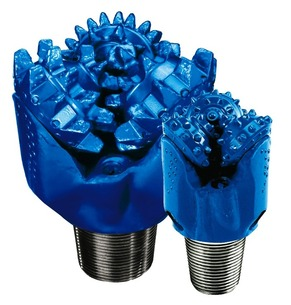
\includegraphics[scale=0.3]{images/Rollerconebits}
\centering 
\caption{A Picture of Roller Cone Bits}
\end{figure}

\textbf{Polycrystalline Diamond Compact Bit:} PDC bit employs no moving parts. 
A PDC bit employs a large number of cutting elements, each called a PDC cutter.The PDC cutter is made 
by bonding a layer of polycrystalline man-made diamond to a cemented tungsten 
carbide substrate in a high pressure, high temperature process. 
The diamond layer is composed of many tiny diamonds which are grown together at random orientation for 
maximum strength and wear resistance.Figure 3.2 shows the image of PDC Bits.

\vspace{1em}

\begin{figure}[h]
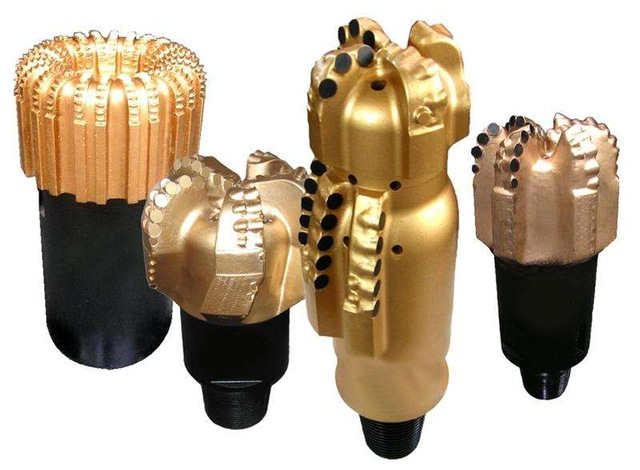
\includegraphics[scale=0.3]{images/PDCbits}
\centering 
\caption{A Picture of PDC Bits}
\end{figure}

\textbf{Diamond Bit:} Diamond is the hardest mineral and also posses the highest thermal conductivity 
of any other mineral allowing it to dissipate heat very quickly. 
These bits are used for drilling hard and
abrasive formations. Diamond bits are manufactured as either drilling or coring bits.



\section{Drilling Mud}
	
Drilling Mud or drilling fluid is a critical component in the rotary drilling processes.

The primary functions of drilling fluids are:

\begin{itemize}

\item Remove cuttings from the wellbore.
\item Prevent formation fluids from entering into the wellbore.
\item Maintain wellbore stability
\item Cool and Lubricate the bit
\item Transmit Hydraulic Horsepower to bit

\end{itemize}

\subsection*{Types of Drilling fluids}

The two major types of mud system used are Oil Based Mud which consists of oil 
as a continuous phase and other is Water Based mud which consists of water as 
a continuous phase.Mostly water based mud is used in Mehsana. The following 
mud systems are in continuous use in Mehsana Asset:

\begin{enumerate}[(a)]

\item SPUD Mud
\item KPPA Mud
\item NDDF Mud

\end{enumerate}

\begin{enumerate}[(a)]

\item \textbf{Spud Mud:}

Mud used to drill a well from the surface to a shallow depth .Onshore spud mud
consists of bentonite clay whereas in offshore guar gum and salt gel are used 
in offshore.

\item \textbf{KPPA Mud:}

It is an abbreviation of KCL, PHPA, polyol mud.KCL and PHPA in the mud acts as 
a shale inhibitor and polyol provides lubricity to the mud.

\item \textbf{NDDF Mud}

It is generally used near pay zone. It is an abbreviation of Non Damaging 
Destructive Fluid which does not uses barite but polymers as a weighing agent as 
barite is non biodegradable and damages the pay zone permeability and porosity.
\end{enumerate}


\noindent \textbf{Field Tests on Drilling Mud}

The mud properties are regularly monitored by mud engineer. These measurements 
will be used to determine if the properties of mud have been deteriorated and 
require treatment or not.

The following tests are used to determine the under mentioned :
\begin{itemize}

\item Mud Density

The density of the drilling mud can be determined with the mud balance shown 
in Figure. The cup of the balance is completely filled with a sample of the
mud and the lid placed firmly on top (some mud should escape through the hole 
in the lid). The balance arm is placed on the base and the rider adjusted until 
the arm is level. The density can be read directly off the graduated scale at 
the left-hand side of the rider.Figure 3.3 shows the image of Mud balance.


\begin{figure}[h]
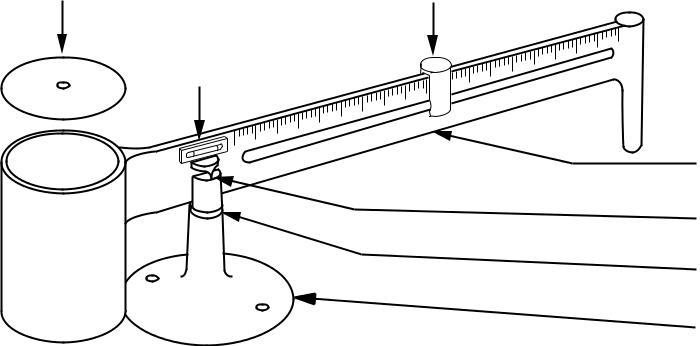
\includegraphics[scale=0.3]{images/mudbalance}
\centering 
\caption{A Picture of Mud Balance}
\end{figure}

\item Viscosity

The rheological character of drilling fluids is discussed at length in the 
chapter on Drilling Hydraulics. In general terms however, viscosity is a 
measure of a liquids resistance to flow. Two common methods are used on the rig 
to measure viscosity.Figure 3.4 shows the image of Marsh Funnel Viscometer.

The marsh funnel viscometer is used to make the quickest analysis of the 
viscosity of drilling fluid .However this device only gives change in 
viscosity and does not quantify rheological properties such as yield point 
and plastic viscosity for which we use rotational viscometer.

Rotational viscometer: The multi-rate rotational viscometer is used
to quantify the rheological properties of the drilling mud. The
assessment is made by shearing a sample of the mud, at a series of
prescribed rates and measuring the shear stress on the fluid at these
different rates.

\begin{figure}[h]
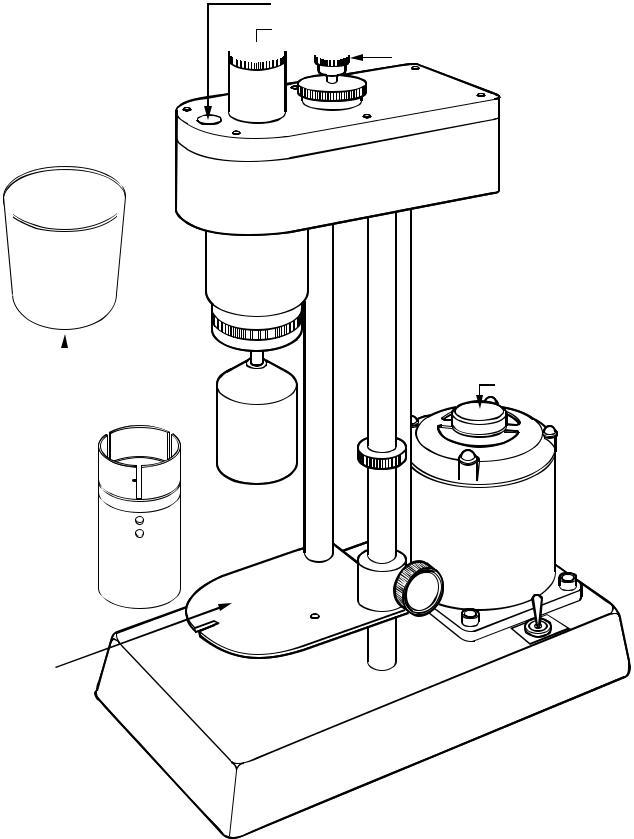
\includegraphics[scale=0.3]{images/marshfunnelvisometer}
\centering 
\caption{A Picture of Marsh Funnel Viscometer}
\end{figure}

\item Gel Strength

The gel strength of the drilling mud can be thought of as the strength of any internal structures which are formed in the mud when it is static. The gel strength of the mud will provide an indication of the pressure required to initiate flow after the mud has been static for some time. The gel strength of the mud also provides an indication of the suspension properties of the mud and hence its ability to suspend cuttings when the mud is stationary . It is measured using rotational viscometer by measuring viscosity at 3rpm and after 10 seconds.

\item Filtration

The filter cake building properties of mud can be measured by means of a filter press. The following are measured during this test :

1. The rate at which fluid from a mud sample is forced through a filter under specified temperature and pressure.

2. The thickness of the solid residue deposited on the filter paper caused by the loss of fluids.

\item pH Determination

The pH of the mud will influence the reaction of various chemicals and must therefore be closely controlled. The pH test is a measure of the concentration of hydrogen ions in an aqueous solution. This can be done either by pH paper or by a special pH meter.

\end{itemize}
 
%mud balance should be added 
%marsh funnel visometer should be added
%pdc and roller cone bits should be added
 
 